\documentclass{astroedu-lab}

\begin{document}

\pagestyle{plain}

\begin{problem}{\huge Лабораторная работа 2.4.1\\\\Скин-эффект\\\\Выполнил Жданов Елисей Б01-205}

\section{Цель работы:}

Исследовать явление проникновение переменного магнитного поля в медный полый цилиндр

\section{Оборудование:}

Генератор сигналов АКИП–3420

Соленоид, намотанный на полый цилиндрический каркас

Медный экран в виде полого цилиндра

Измерительная катушка

Амперметр

Вольтметр

Двухканальный осциллограф GOS–620

RLC-метр

\section{Теоретическая справка}

\begin{figure}[!h]
	\centering
	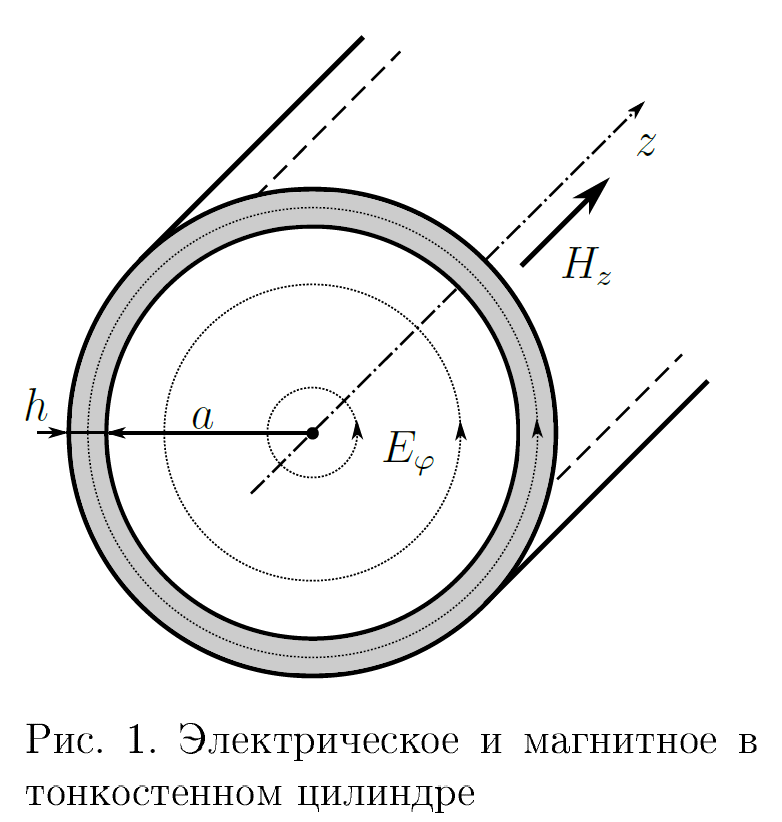
\includegraphics[width=0.4\textwidth]{уст1.png}
	\label{fig:boiler}
\end{figure}


В работе изучается скин-эффект в длинном тонкостенном медном цилиндре, помещённом внутрь соленоида.

Теоретически такая задача сложнее, чем рассмотренный в п.3.1 (см. Лабораторный практикум по общей физике: электричество и магнетизм, раздел 7) скин-эффект в полубесконечном пространстве: здесь требуется совместное решение уравнений скин-эффекта (уравнения диффузии поля) (л7.22), (л7.23)* в стенке цилиндра и квазистационарных уравнений поля в его полости.

Пусть цилиндр достаточно длинный, так что
в нём можно пренебречь краевыми эффектами. В
этом приближении магнитное поле H всюду направлено
по оси системы (ось z), а вихревое электрическое
поле $\boldsymbol{E}$ будет всюду перпендикулярно радиусу, то есть линии поля образуют соосные окружности (рис. 1). Все величины будем считать колеблющимися по гармоническому закону с некоторой частотой $\omega$, задаваемой частотой колебания тока в соленоиде. Тогда для ненулевых компонент поля можно записать
$$
H_z=H(r) e^{i \omega t}, \quad E_{\varphi}=E(r) e^{i \omega t},
$$

где $H(r)$ и $E(r)$ комплексные амплитуды колебаний соответствующих полей, зависящие только от Рис. 1. Электрическое и магнитное в расстояния $r$ до оси системы. Заметим, что на гра- тонкостенном цилиндре нице цилиндра должны быть непрерывны касательные к поверхности компоненты как $\boldsymbol{E}$, так и $\boldsymbol{B}$, поэтому функции $E(r)$ и $H(r)$ непрерывны во всей исследуемой области.

Пусть длинный полый цилиндр имеет радиус $a$ и толщину стенки $h \ll a$. Последнее условие позволяет для описания поля внутри стенки ограничиться одномерным приближением. При этом для полного решения задачи необходимо вычислить и распределение поля внутри цилиндра.

Поскольку внутри цилиндра ток отсутствует, магнитное поле там является однородным (аналогично полю внутри пустого соленоида): $H_z(r, t)=H_1 e^{i \omega t}$, где $H_1=\mathrm{const} \quad$ амплитуда поля на внутренней поверхности цилиндра. Для нахождения вихревого электрического поля воспользуемся законом электромагнитной индукции (л7.3) в интегральной форме:
$$
E_{\varphi} \cdot 2 \pi r=-\mu_0 \pi r^2 \cdot \frac{d H_z}{d t} \quad \rightarrow \quad E(r)=-\frac{1}{2} \mu_0 r \cdot i \omega H_1 .
$$

Отсюда получим связь амплитуд колебаний электрического и магнитного полей на внутренней $(r=a)$ границе цилиндра:
$$
E_1=-\frac{1}{2} i \omega a \mu_0 H_1
$$

\begin{figure}[!h]
	\centering
	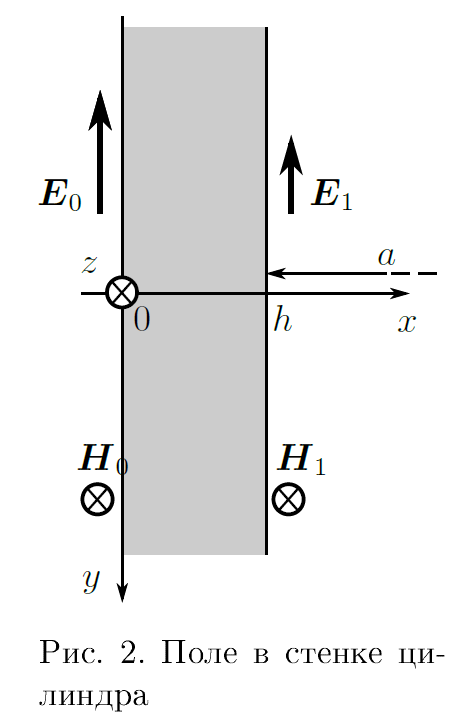
\includegraphics[width=0.25\textwidth]{уст2.png}
	\label{fig:boiler}
\end{figure}

Соотношение (1) используем далее как дополнительное граничное условие для задачи о распределении поля внутри стенки.
Поле внутри тонкой стенки цилиндра ( ээкрана») описывается уравнением скин-эффекта (л7.25) (уравнением диффузии поля) в плоской геометрии (рис. 2). Поместим начало отсчёта на внешнюю поверхность цилиндра и направим ось $x$ к оси системы, и аналогично (л7.26) запишем дифференциальное уравнение для комплексной амплитуды магнитного поля:
$$
\frac{d^2 H}{d x^2}=i \omega \sigma \mu_0 H
$$
(для медного цилиндра можно положить $\mu \approx 1$ ).
Граничные условия для (2) зададим в виде
$$
H(0)=H_0, \quad H(h)=H_1 .
$$

Здесь $H_0 \quad$ амплитуда колебаний магнитного поля на внешней границе цилиндра. Её значение определяется только током в облиндра мотке соленоида, и совпадает с полем внутри соленоида в отсутствие цилиндра. Величина $H_1$ также поддаётся непосредственному измерению это амплитуда колебаний однородного поля внутри цилиндра. Поля $H_0$ и $H_1$ не являются независимыми они связаны через решение уравнений поля вне проводника, т. е. внутри «экрана». Эта связь выражена соотношением (1).

Решение (2) ищем в виде
$$
H(x)=A e^{\alpha x}+B e^{-\alpha x},
$$

где $A, B$ определяемые из граничных условий константы,
$$
\alpha=\sqrt{i \omega \sigma \mu_0}=\frac{1+i}{\delta}=\frac{\sqrt{2}}{\delta} e^{i \pi / 4}
$$

- один из корней уравнения (л7.28), $\delta$ глубина скин-слоя
$$
\delta=\sqrt{\frac{2}{\omega \sigma \mu_0}} .
$$

Заметим, что это решение немного отличается от (л7.29) : ранее мы использовали только один корень уравнения (л7.28), однако здесь мы имеем дело уже не с полупространством, а с конечной областью в виде плоского слоя $h$, поэтому решение должно содержать оба корня.
Первое условие (3) даёт $A+B=H_0$, что позволяет исключить $A$ из (4):
$$
H(x)=H_0 e^{-\alpha x}+2 B \operatorname{sh} \alpha x .
$$

Выразим электрическое поле из закона Ампера (л7.21). В одномерном случае
$$
E(x)=\frac{1}{\sigma} \frac{d H}{d x}=\frac{\alpha}{\sigma}\left(-H_0 e^{-\alpha x}+2 B \operatorname{ch} \alpha x\right) .
$$





Далее положим $x=h$, воспользуемся условием (1), и, исключив константу $B$, получим после преобразований связь между $H_0$ и $H_1$ :
$$
H_1=\frac{H_0}{\operatorname{ch} \alpha h+\frac{1}{2} \alpha a \operatorname{sh}(\alpha h)} .
$$

Рассмотрим предельные случаи (7).
1. При малых частотах толщина скин-слоя превосходит толщину цилиндра $\delta \gg h$. Тогда $|\alpha h| \ll 1$, поэтому $\operatorname{ch} \alpha h \approx 1$, sh $\alpha h \approx \alpha h$ и
$$
H_1 \approx \frac{H_0}{1+i \frac{a h}{\delta^2}}
$$

Заметим, что величина $a h / \delta^2$ в общем случае не мала, поскольку при $h \ll a$ возможна ситуация $h \ll \delta \ll a$. Отношение модулей амплитуд здесь будет равно
$$
\frac{\left|H_1\right|}{\left|H_0\right|}=\frac{1}{\sqrt{1+\left(\frac{a h}{\delta^2}\right)^2}}=\frac{1}{\sqrt{1+\frac{1}{4}\left(a h \sigma \mu_0 \omega\right)^2}} .
$$

При этом колебания $H_1$ отстают по фазе от $H_0$ на угол $\psi$, определяемый равенством
$$
\operatorname{tg} \psi=\frac{a h}{\delta^2} .
$$
2. При достаточно больщих частотах толщина скин-слоя станет меньше толщины стенки: $\delta \ll h$. Тогда $|\alpha h| \gg 1$ и $|\alpha a| \gg 1$, а также $\operatorname{sh}(\alpha h) \approx \operatorname{ch}(\alpha h) \approx \frac{1}{2} e^{\alpha h}$. Выражение $(7)$ с учётом (5) переходит в
$$
\frac{H_1}{H_0}=\frac{4}{\alpha a} e^{-\alpha h}=\frac{2 \sqrt{2} \delta}{a} e^{-\frac{h}{\delta}} e^{-i\left(\frac{\pi}{4}+\frac{h}{\delta}\right)} .
$$

Как видно из формулы $(11)$, в этом пределе поле внутри цилиндра по модулю в $\frac{2 \sqrt{2} \delta}{a} e^{-h / \delta}$ раз меньше, чем снаружи, и, кроме того, запаздывает по фазе на
$$
\psi=\frac{\pi}{4}+\frac{h}{\delta}=\frac{\pi}{4}+h \sqrt{\frac{\omega \sigma \mu_0}{2}} .
$$

На рис. 3 схематично изображено распределение магнитного поля от координаты в двух рассмотренных предельных случаях.

\section{Экспериментальная установка}

\begin{figure}[!h]
	\centering
	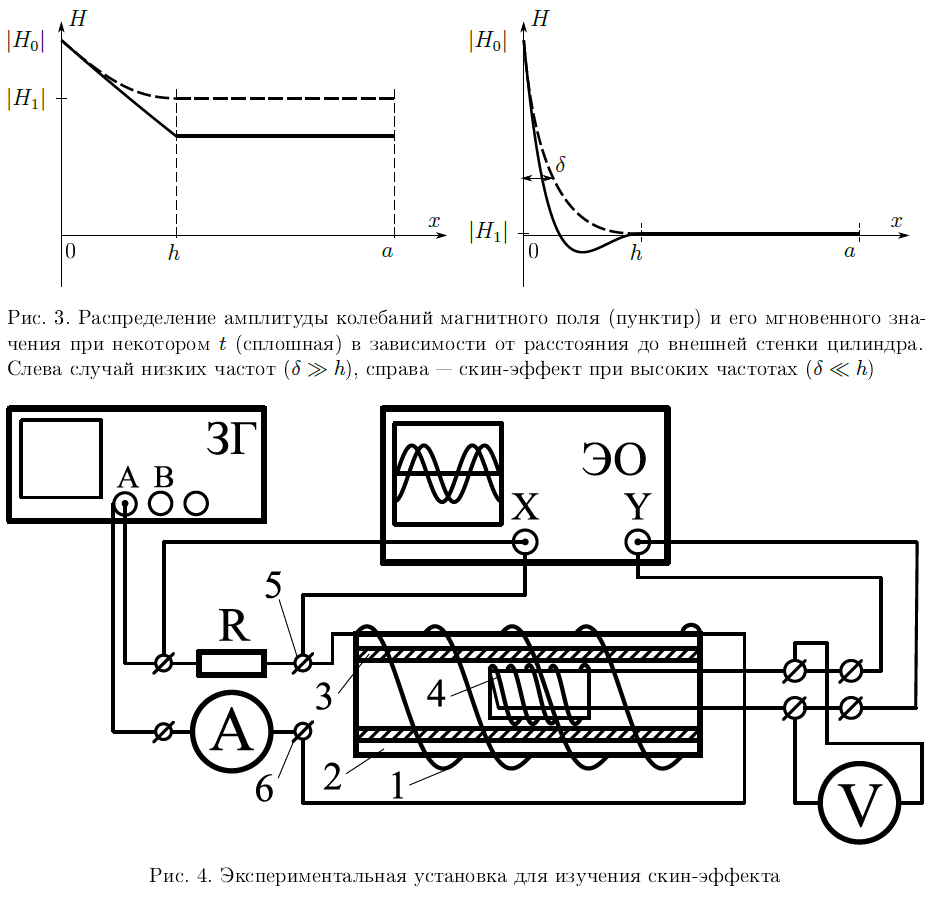
\includegraphics[width=1\textwidth]{уст3.png}
	\label{fig:boiler}
\end{figure}

Схема экспериментальной установки для исследования скин-эффекта в полом цилиндре изображена на рис. 4.

Переменное магнитное поле создается с помощью соленоида 1, намотанного на цилиндрический каркас 2 из поливинилхлорида, который подключается к генератору сигналов (ЗГ) АКИП-3420 (канал А). Внутри каркаса расположен медный экран 3 в виде полого цилиндра (актуальные параметры экрана указаны на установке).

Действующее значение переменного тока в цепи соленоида измеряется цифровым амперметром «А». Действующее значение переменного напряжения на измерительной катушке 4 измеряется цифровым вольтметром «V». В качестве амперметра и вольтметра используются два мультиметра GDM-8245.

Для измерения сдвига фаз между током в цепи соленоида и напряжением на измерительной катушке используется двухканальный осциллограф GOS-620 (ӨО). На канал «Y» осциллографа подается напряжение с измерительной катушки, а на канал «X» —
напряжение с резистора R, которое пропорционально току в цепи соленоида.
Схема экспериментальной установки для нахождения проводимости $\sigma$ по изменению
индуктивности катушки L изображена на рис. 5. RLC-метр, измеряющий индуктивность,
подключается к катушке 1 через клеммы 5 и 6 на панеле установки. Другие приборы при
этом должны быть отсоединены от цепи, т.к. RLC-метр измеряет индуктивность активным
образом.

\section{Измерение отношения амплитуд магнитного поля внутри и вне экрана}


\begin{figure}[!h]
	\centering
	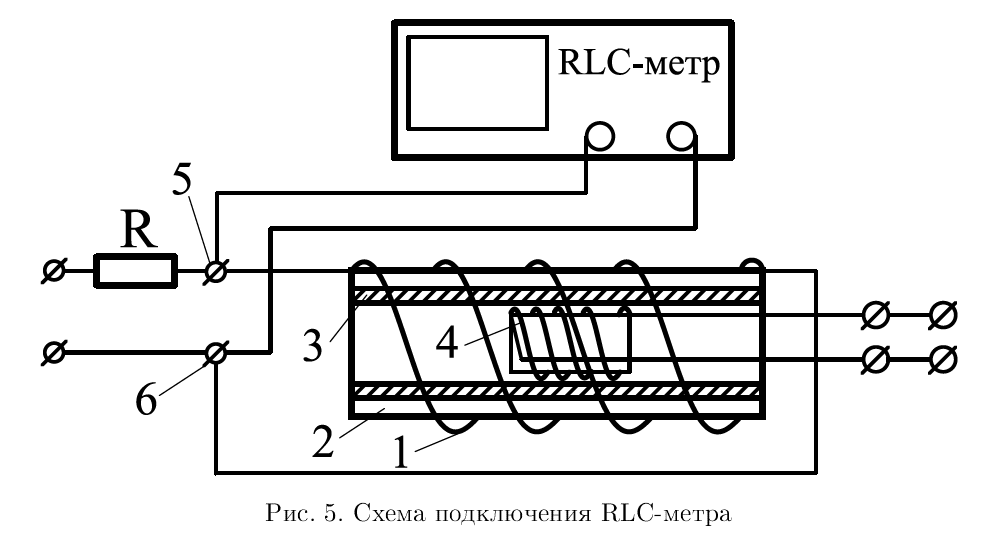
\includegraphics[width=1\textwidth]{уст4.png}
	\label{fig:boiler}
\end{figure}

С помощью вольтметра V измеряется действующее значение ЭДС индукции, которая
возникает в измерительной катушке, находящейся в переменном магнитном поле $H_1 e^{i \omega t}$.
Комплексная амплитуда ЭДС индукции в измерительной катушке равна
\begin{equation}
	U = - S N \frac{d B_1(t)}{dt} = -i \omega \mu_0 S N H_1 e^{i \omega t}
\end{equation}

где $S N$ - произведение площади витка на число витков измерительной катушки. Показания вольтметра, измеряющего это напряжение:
$$
U=\frac{S N \omega}{\sqrt{2}} \mu_0\left|H_1\right| .
$$

Видно, что модуль амплитуды магнитного поля внутри экрана $\left|H_1\right|$ пропорционален $U$ и обратно пропорционален частоте сигнала $\nu=\omega / 2 \pi$
$$
\left|H_1\right| \propto \frac{U}{\nu} .
$$

При этом поле вне экрана $\left|H_0\right|$ пропорционально току $I$ в цени соленоида, измеряемому амперметром $A$ :
$$
\left|H_0\right| \propto I .
$$

Следовательно,
$$
\frac{\left|H_1\right|}{\left|H_0\right|}=\text { const } \cdot \frac{U}{\nu I}
$$

Таким образом, отношение амплитуд магнитных полей снаружи и вне экрана (коэф фициент ослабления) может быть измерено по отношению $U / \nu I$ ири разных частотах Неизвестная константа в соотношении (13) может быть определена по измерениям при малых частотах $\nu \rightarrow 0$, когда согласно (9) $\left|H_1\right| /\left|H_0\right| \rightarrow 1$.

\section{Определение проводимости материала экрана по фазовому сдвигу}

В установке в качестве экрана используется медная труба промышленного ироизвод ства. Технология изготовления труб оказывает заметное влияние на электропроводимость. Из-за наличия примесей проводимость меди нашей трубы отличается от табличного значе ния (в меньшую сторону). Для определения $\sigma$ нашего экрана предлагается использовать экрана при низких частотах и зависимость (12 - при высоких частотах.

Из формул (10) и (6) следует линейная зависимость $\operatorname{tg}(\psi)$ от $\nu$, причем апироксимиру ющая ирямая должна ироходить через начало координат.

Как видно из выражения (12), в области больших частот $\nu \gg 1 /\left(\pi h^2 \sigma \mu_0\right)$ зависимость $(\psi(\sqrt{\nu})-\pi / 4)$ апшроксимируется прямой, шроходящей через начало координат. По наклону этих ирямых можно вычислить проводимость материала экрана.
$\underline{8}$
Процедура измерения разности фазс помоцью осцилюграфа подробно оиисана в При ложении $\Gamma$

Заметим, что на схеме, изображённой на рис. 4 на входной канал У осцилюграфа пода ётя сигнал с измерительнй катушки, когорый иронориионаен не иолю внутри экрана. а его производной по времени, а это означнет, что появляется дополнительный сдвиг по нусоидами будет на $\pi / 2$ больше фазового сдвига между магнитными иолями вне и внугри экрана:
$$
\varphi=\psi+\frac{\pi}{2}
$$

\section{Влияние скин-эффекта на индуктивность катушки}

Из-за скин эффекта индуктивность соленоида с медным цилиндрическим экраном внутри будет зависеть от частоты тока. На высоких частотах магнитное поле не проника ет внутрь соленоида (за экран), поэтому суммарный магнитный поток, иронизывающий катушку, уменьшается, и, соответственно, уменьшается и индуктивность. При низких частотах когда толщина скин-слоя $\delta$ больше толщины медного экрана h, магнитное поле
проникает внутрь катушки, однако его амплитуда падает (по формуле (9)) и возникает разность фаз между колебаниями поля за экраном и перед ним (по формуле (10). Из-за чего также изменяется магнитный пюток, а следовательно - и индуктивность.

Рассмотрим магнитный поток через катушку как сумму двух магнитных потоков: 1) пронизывающий область за экраном $\Phi_{\text {in: }}$ :
$$
\Phi=\Phi_{\text {out }}+\Phi_{\text {in }}=H_0 S_0+H_1 S_1=L I,
$$

где $H_0, H_1-$ мгновенные значения магнитного поля внутри и снаружи цилиндра ири данном токе $I ; S_0, S_1$ - площади внешней и внутренней (по отношению к цилиндрическому экрану) областей соответственно.

Очевидно, что минимальная индуктивность будет в случае, когда $\Phi_{\text {in }}=0$ (поле есть только во внешней области). При этом $L_{\min }$ не зависит от частоты:
$$
L_{m i n}=\frac{\Phi_{\text {out }}}{I} .
$$

Выразим поток магнитного поля сквозь внутреннюю область $\Phi_{\text {in }}$ через поток сквозь внешнюю $\Phi_{\text {out }}$ при ироизольном переменном токе I:
$$
\Phi_{\text {in }}=H_1 S_1=\frac{H_1 S_1}{H_0 S_0} \Phi_{\text {out }}=\frac{\Phi_{\text {out }}}{n} \frac{S_1}{S_0}
$$

где коэффициент $n$, характеризуюций ослабление поля за экраном, равен:
$$
n=\frac{H_0}{H_1}=\frac{\left|H_0\right|}{\left|H_1\right|} \frac{1}{\cos \psi},
$$

Максимальная индуктивность катушки достигается при максиманьном потоке поля ра внутренней области (когди $\left.H_0=H_1\right)$ :
$$
\Phi_{\max }=\Phi_{\text {out }}+\Phi_{\text {in } \max }=H_0\left(S_0+S_1\right)=L_{\max } I_m,
$$

где поток через внешнюо область равен $H_0 S_0=L_{\operatorname{man}} I_m$. Откуда получнем отнонени плоцадей областей:
$$
\frac{S_1}{S_0}=\frac{L_{\max }-L_{\min }}{L_{\min }} .
$$

Суммируя всё выненаписанное
$$
L=L_{\min }+\frac{L_{\max }-L_{\min }}{n} .
$$

Используя формулы (9, 10, 6) окончательно получаем зависимость индуктивности катушки от частоты:

$$
\begin{aligned}
&  \\
& \frac{L_{\max }-L}{L-L_{\text {min }}}=\left(\pi a h \mu_0 \sigma \nu\right)^2 \text {. } \\
& 
\end{aligned}
$$
Данная зависимость может быть аппроксимирована прямой, по углу наклона которой можно найти проводимость материала экрана $\sigma$

\section{Измерения, Обработка}

Внутренний диаметр катушки составляет 45 мм, толщина - 1.5 мм.

1) Частота $\nu_h$ составляет

\begin{equation}
	\nu_h  = \frac{2}{\delta^2 \sigma \mu_0} = 2.25 \text{ кГц}
\end{equation}

2-5) Запустим установку и произведем изменения во всех указанных диапазонах, сводя все данные в единую электронную таблицу

7) В области частот $\nu \ll \nu_h$ $\alpha h \ll 1$, и из (7) получаем
\begin{equation*}
    {(c\xi)}^2 \approx \frac{1}{1+A\nu^2}
\end{equation*}
или, эквивалентно
\begin{equation*}
    \frac{1}{\xi^2}=B\nu^2 + c^2 \text{ где } B=\pi a h \sigma \mu_0 c
    \label{eq:liniya_dlya_c}
\end{equation*}

\begin{center}
	\Large $\frac{1}{\xi^2}(\nu^2)$
\end{center}

\begin{figure}[!h]
	\centering
	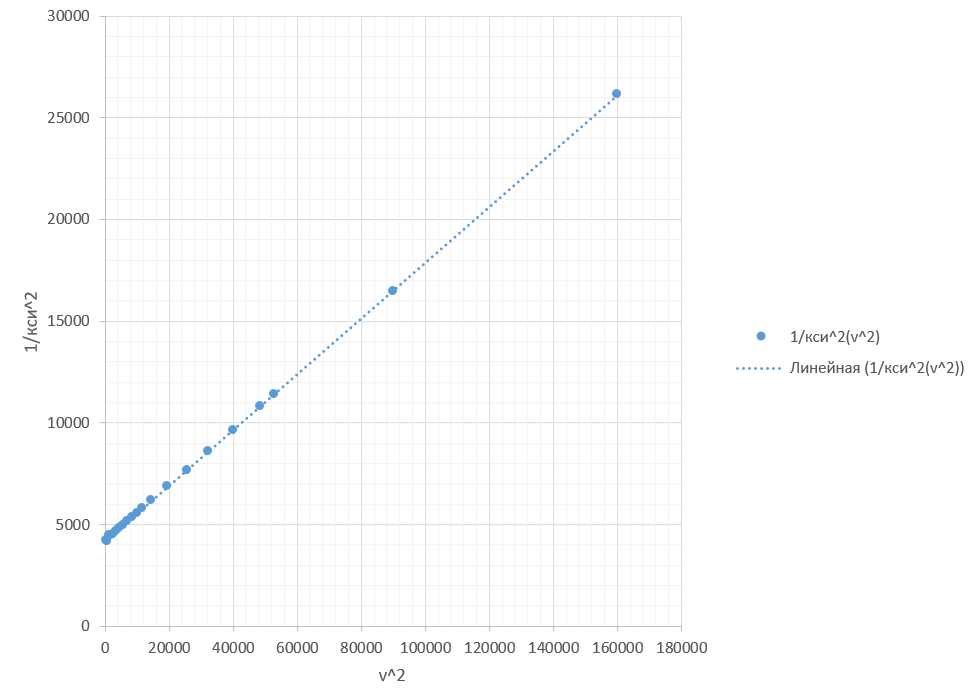
\includegraphics[width=1\textwidth]{гр1.png}
	\label{fig:boiler}
\end{figure}

Найдем угловые коэффициенты прямых для каждой установки по МНК.

\[
	a = \frac{<x_i y_i> - < x > < y_i >}{< x_i^2> - < x_i >^2}
\]

\[
	b = < \nu_i > - a < N_i >
\]

Также рассчитаем их погрешности

\begin{equation}
	S_a^2 = \frac{< x_i^2>}{< x_i^2 > - < x_i >^2} \cdot \frac{<  b_i - b > ^2}{n - 2}
\end{equation}

\begin{equation}
	y = (a \pm S_a) + (b \pm S_b) \cdot x = (4183 \pm 11) + (0.13708 \pm 0.00023) \cdot x
\end{equation}

Зависимость линейная

Коэффициент пропорциональности

\begin{equation}
	\xi_0[|H_1/H_0| = 1] = \frac{1}{\sqrt{a}} = 0.1546 \pm 0.0002
\end{equation}

Проводимость

\begin{equation}
	\sigma = \frac{B}{\pi a h \mu_0 c} = (51.70 \pm 0.16) \cdot  10^6 \frac{\text{См}}{\text{м}}
\end{equation}

8) Зависимость фазового сдвига от частоты

\newpage

a) Линейная часть

\begin{figure}[!h]
	\centering
	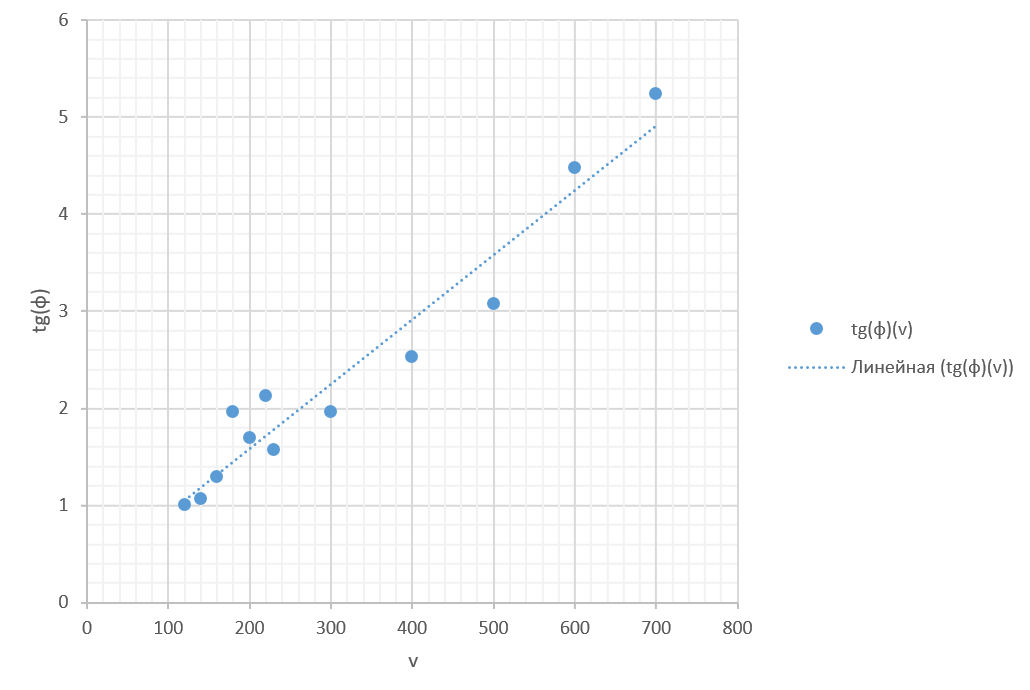
\includegraphics[width=1\textwidth]{гр3.png}
	\label{fig:boiler}
\end{figure}

\newpage

б) Нелинейная часть

\begin{figure}[!h]
	\centering
	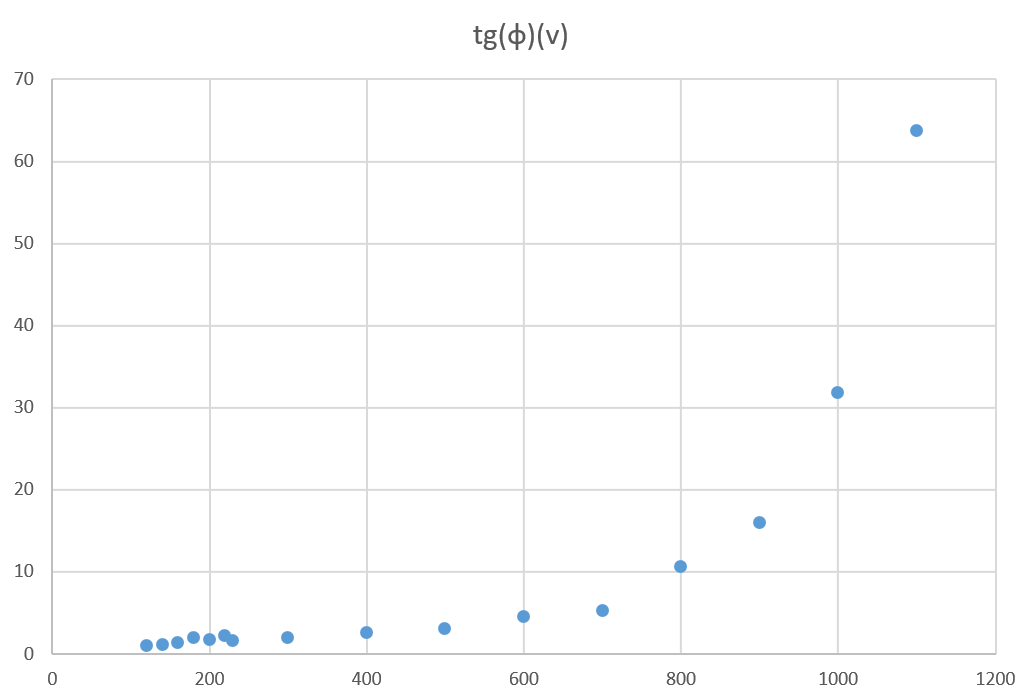
\includegraphics[width=1\textwidth]{гр2.png}
	\label{fig:boiler}
\end{figure}

Линеаризация для первого графика

\begin{equation}
	y = (a \pm S_a) + (b \pm S_b) \cdot x = (0.25 \pm 0.19) + (0.00666 \pm 0.00053) \cdot x
\end{equation}

Тогда поскольку $tan(\psi) = k \cdot \nu, k = \pi a h \sigma \mu_0$, то проводимость

\begin{equation}
	\sigma = \frac{b}{\pi a h \mu_0} = (50 \pm 4) \cdot 10^7 \frac{\text{См}}{\text{м}}
\end{equation}

9) График зависимости $\psi - \pi/4(\sqrt{\nu})$ для высоких частот

\newpage

\begin{figure}[!h]
	\centering
	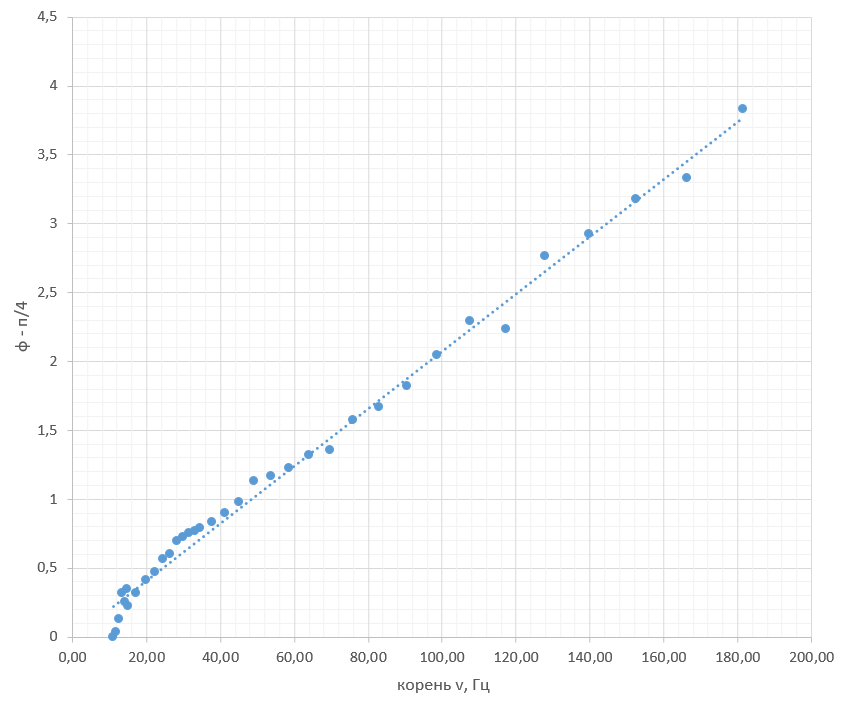
\includegraphics[width=1\textwidth]{гр4.png}
	\label{fig:boiler}
\end{figure}

Зависимость, начиная с частоты $\nu \approx \nu_h$ - линейная.

Линеаризация дает

\begin{equation}
	y = (a \pm S_a) + (b \pm S_b) \cdot x = (0.025 \pm 0.048) + (0.02045 \pm 0.00045) \cdot x
\end{equation}

По формуле 8 $\psi - \pi/4 = k \sqrt{\nu}, k = h \sqrt{\pi \mu_0 \sigma}$

Из графика проводимость 

\begin{equation}
	\sigma = \frac{b^2}{\pi h^2 \mu_0} = (4.7 \pm 0.2) \cdot 10^7 \frac{\text{См}}{\text{м}}
\end{equation}

10) Зависиммость индуктивности от частоты

$$
\begin{aligned}
&  \\
& \frac{L_{\max }-L}{L-L_{\text {min }}}=\left(\pi a h \mu_0 \sigma \nu\right)^2 \text {. } \\
& 
\end{aligned}
$$

Построим график зависимости $L(\nu)$

\begin{figure}[!h]
	\centering
	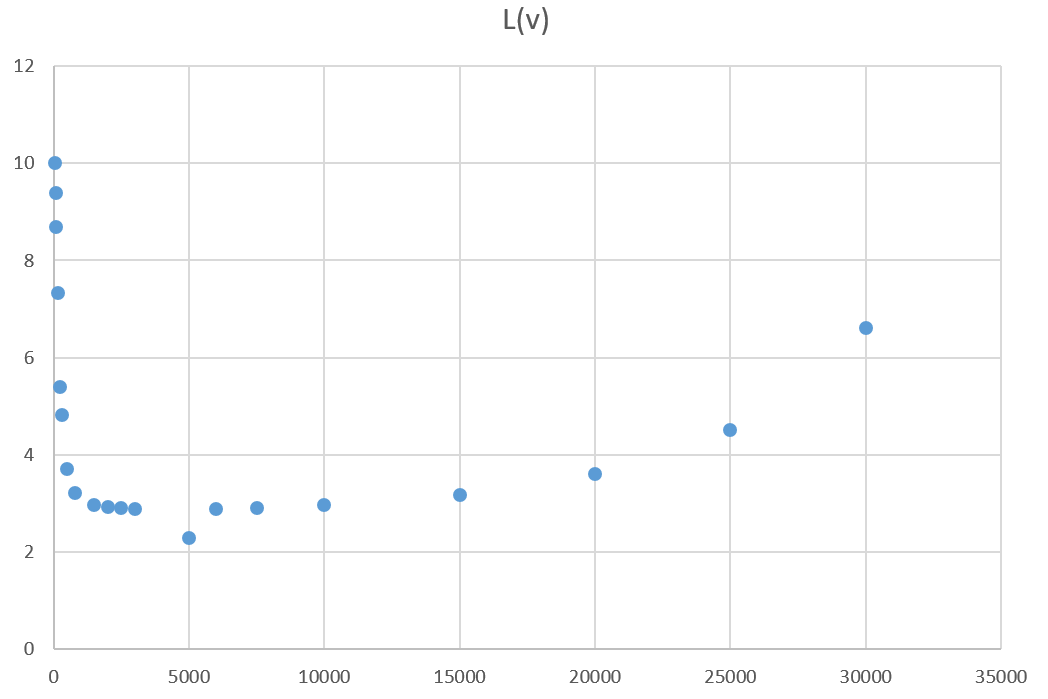
\includegraphics[width=1\textwidth]{гр5.png}
	\label{fig:boiler}
\end{figure}

Максимальная индуктивность $L_{max} = 10.013
 \text{ мГн}$, а минимальная $L_{min} = 2.895 \text{ мГн}$. 

Построим график зависимости $\frac{L_{\max }-L}{L-L_{\text {min }}}(\nu^2)$ при малых частотах

\begin{figure}[!h]
	\centering
	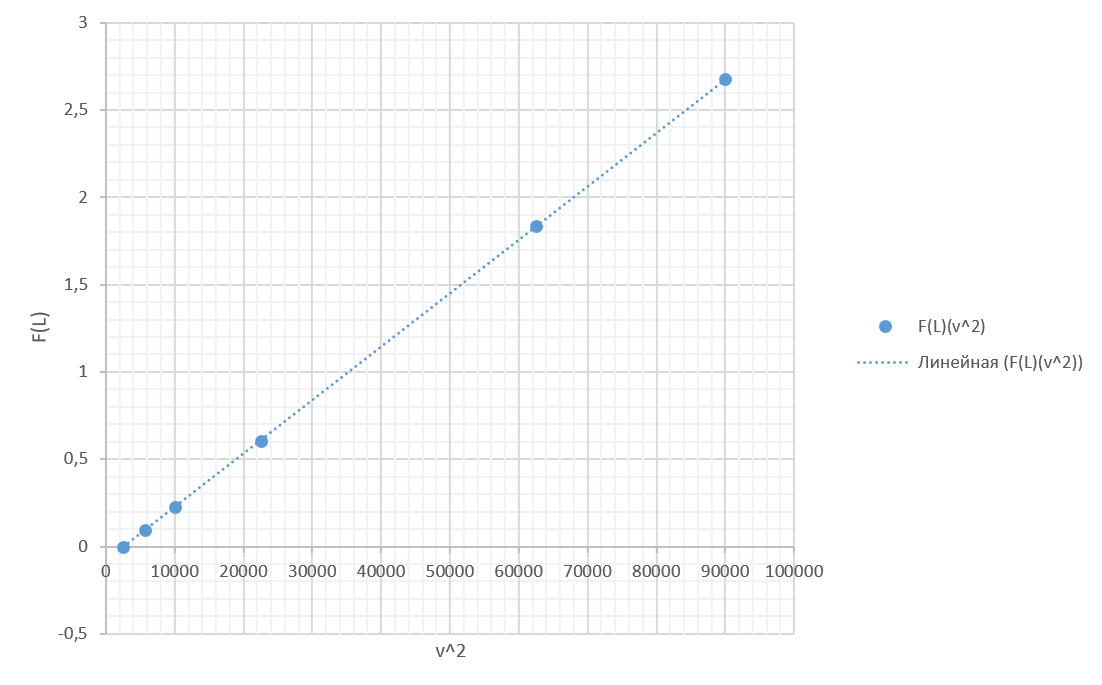
\includegraphics[width=1\textwidth]{гр6.png}
	\label{fig:boiler}
\end{figure}

Линеаризация

\begin{equation}
	y = (a \pm S_a) + (b \pm S_b) \cdot x = (-0.0785 \pm 0.0015) + (0.000030614 \pm 3.2e-8) \cdot x
\end{equation}

Проводимость составляет

\begin{equation}
	\sigma = \frac{\sqrt{b}}{\pi a h \mu_0} = (41.53 \pm 0.02) \cdot 10^7 \frac{\text{См}}{\text{м}}
\end{equation}

11) Сведем проводимости в таблицу

.

\begin{table}[!h]
\begin{center}
\begin{tabular}{lrrr}
Метод измерения & $\sigma, 10^{7} \text{См/м}$ & $\Delta\sigma, 10^{7} \text{См/м}$ & $\varepsilon_{\sigma}$\\
\toprule
Отношение амплитуд & 5.170 & 0.016 & 0.31\%\\
Разности фаз (низкие частоты) & 5.0 & 0.4 & 8\%\\
Разности фаз (высокие частоты) & 4.7 & 0.2 & 4.3\%\\
Индуктивность & 4.153 & 0.002 & 0.0048\%\\

\end{tabular}
\end{center}
    \caption{Сравнение результатов различных методов}\label{}
\end{table}

Приведу также отношение $\frac{H_1}{H_0}$

\begin{figure}[!h]
	\centering
	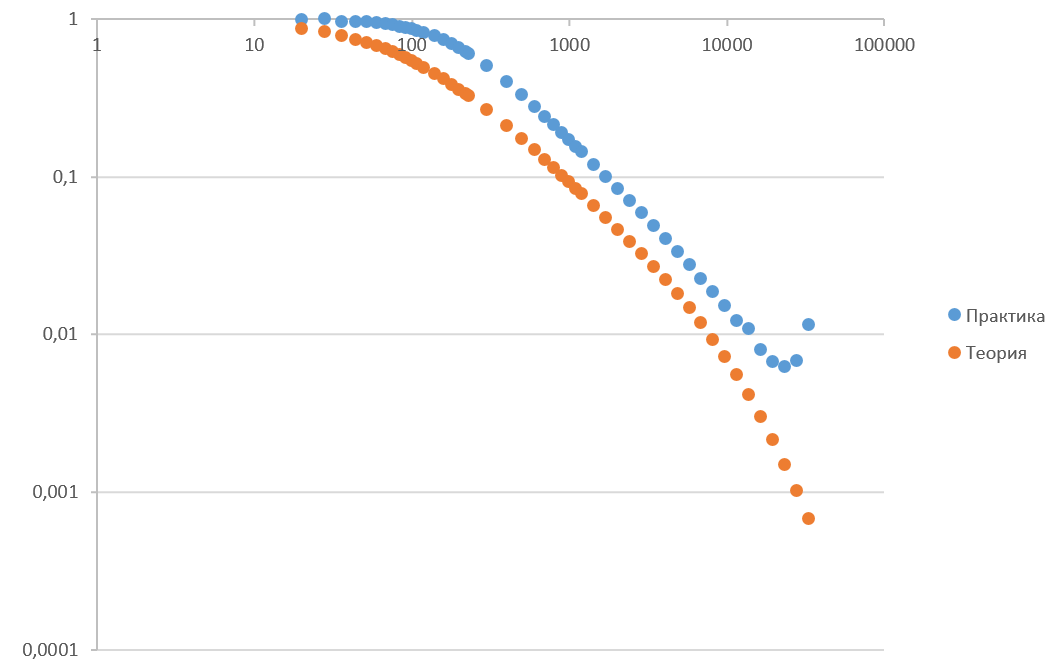
\includegraphics[width=1\textwidth]{гр7.png}
	\label{fig:boiler}
\end{figure}

\section{Вывод}

Теоретическая зависимость довольно хорошо совпадает с практической. Отклонения на начале и конце зависимостей друг от друга обусловлены неточностью теоретической модели, в результате которой качественно поведение при экстремальных частотах отличается.

\section{Ресурсы}

Расчет по МНК: метод-наименьших-квадратов.рф


\end{problem}
\end{document}